\setchapterpreamble[u]{\margintoc}
\chapter{Cuantización del campo escalar libre}
\labch{Part}

\begin{center}
  \large Todo esto lo he sacado del \cite{Dobdado}
\end{center}
\section{EL campo electromagnético clásico}
\section{Invariancia Gauge}

Supongamos una transformación del tipo:
$$ A^\mu(x) \rightarrow A'^\mu(x) = A^\mu(x) - \partial^\mu \Lambda(x) $$
y

$$ F^{\mu\nu} \rightarrow F'^{\mu\nu} = F^{\mu\nu} $$

$$
\begin{align*}
    &\partial_\mu F^{\mu\nu} = 0 \quad \Box \mathbf{A}^\nu - \partial^\nu (\partial_\mu A^\mu) = 0
\end{align*}
$$

De ahora en adelante, suponemos que nuestro campo cumple el gauge transverso y el gauge temporal:

$$ 
\begin{align*}
    \partial_\mu A^\mu &= 0 \quad (\text{Ec. de onda}) \\
    A^0 &= 0 \\
    \nabla \cdot \mathbf{A} &= 0
\end{align*}
$$

Si $\Box \Lambda = 0$, $\partial^\mu A'_\mu = \partial^\mu A_\mu - \Box \Lambda = 0$ entonces $\Box \Lambda = 0$, $\partial^\mu A_\mu = 0$, $\nabla \cdot \mathbf{A} = 0$.

Al hacer esto, hay que tener en cuenta que las transformaciones no sean invariantes, por lo que las ecuaciones no son covariantes.

$$
\begin{align*}
    \int \partial^0 A^0 &= \int d \phi \\
    \Box A^\mu &= 0 \\
    \partial^j \phi &= \phi^0 \quad A^0 \rightarrow -\phi = A'_\mu = A_\mu + \partial_\mu \Lambda = 0
\end{align*}
$$

Escogemos 
$$
\begin{align*}
    \phi &= 0 \quad A^\mu = \nabla \cdot \mathbf{A} 
\end{align*}
$$
Teniendo en cuenta que $ \partial_\mu F^{\mu\nu} = 0 $

De esta forma obtenemos que

$$
T^{\mu\nu} = F^{\mu\lambda} F^{\nu}_{\phantom{\nu}\lambda} + \frac{1}{4} g^{\mu\nu} F_{\rho\sigma} F^{\rho\sigma} 
$$

$$
\begin{cases}
T^{\mu\nu} - T^{\nu\mu} \\
\partial_\mu T^{\mu\nu} = 0
\end{cases}
$$

$$ 
T^{00} = H = \int (\mathbf{E}^2 + \mathbf{B}^2) \, dx \equiv \text{Energía}
$$

$$
T^{0i} = P = \int (\mathbf{E} \times \mathbf{B}) \, dx \equiv \text{Momento lineal}
$$

$$
\Pi^0 = \frac{\delta \mathcal{L}}{\delta(\partial_0 A^0)} = 0
$$

No aparece $ A^0 $, aparece $-\frac{1}{4} F_{\mu\nu} F^{\mu\nu}$ y $ F^{00} = 0 $.

Los gauge no son simétricos, son redundancias producto de hacer las ecuaciones invariantes relativistas, ya que añadimos 2 grados de libertad ficticios para asegurar la covariancia. Si imponemos los gauge, las ecuaciones ya no son covariantes, y por tanto no son invariantes relativistas, pero ya no hay grados de libertad ficticios.

$$
-A^i = A_i \quad \Rightarrow \quad \Pi^i = E^i
$$

$$
A_i \quad \Rightarrow \quad H = \frac{\delta \mathcal{L}}{\delta(\partial_0 A_i)} \quad \Rightarrow \quad -F^{0i} = E^i
$$
\section{Cuantización del Gauge de radiaición}
$$
A^0 = 0 \quad \Rightarrow \quad \begin{cases}
\nabla \cdot \mathbf{A} = 0 \\
\Box \mathbf{A}^\mu = 0
\end{cases}
$$

Ahora las ecuaciones no son invariantes relativistas, pero trabajamos con los grados de libertad físicos.

$$
\hat{A}^0 \neq \hat{A}^0
$$

Pasamos a operadores

$$
\hat{A} = \hat{A}^+ + \hat{A}^-
$$

$$
\mathbf{K} \cdot \mathbf{\hat{E}}(\mathbf{K}, \lambda) = 0
$$

$$
K^0 < 0 
$$

$$
K^2 = \mathbf{K}^2 + \omega^2 = 0 \quad \text{con} \quad \omega = |\mathbf{K}|
$$

$$
\hat{\mathbf{A}} = 0 \quad \Rightarrow \quad \overline{\mathbf{A}}(\mathbf{x},t) = \int d^3K \sum_\lambda \left( \mathbf{E}(\mathbf{K}, \lambda) \hat{a}_{\mathbf{K},\lambda} e^{-i\mathbf{kx}} + \overline{\mathbf{E}}(\mathbf{K},\lambda) \hat{a}^\dagger_{\mathbf{K},\lambda} e^{i\mathbf{kx}} \right)
$$

$$
A^\mu - A^\nu - A^\lambda - A^\rho = 0 
$$

Gauge de radiación

$$
\begin{cases}
\text{Gauge temporal} & \phi = A^0 = 0 \\
\text{Gauge de Coulomb} & \nabla \cdot \mathbf{A} = 0 \\
\text{Gauge de Lorenz} & \partial_\mu A^\mu = 0
\end{cases}
$$

$$
\Box A^\mu = 0
$$

$$
A^\mu = \Lambda^\mu = \int \int dK \left( \mathbf{E}(\mathbf{K}, \lambda) \hat{a}_{\mathbf{K},\lambda} e^{-i\mathbf{kx}} + \overline{\mathbf{E}}(\mathbf{K},\lambda) \hat{a}^\dagger_{\mathbf{K},\lambda} e^{i\mathbf{kx}} \right)
$$

Solución más general a la ecuación de onda $\Box \Lambda^\mu = 0$

La condición del gauge de Coulomb nos pone una condición en $\mathbf{E}(\mathbf{K}, k)$ y $\mathbf{A}$ ya que al derivar respecto a $x$ aparecen términos 

Para que se cumpla la condición

$$
\mathbf{E}(\mathbf{K}, \lambda) \cdot \mathbf{E}(\mathbf{K}, \nu) = \delta_{\lambda\nu}
$$

Con $\mathbf{K} = w \, e_3$, con esta elección cumplimos la condición 

Esto recibe el nombre de "base de polarización lineal"

$ \{e_1, e_2, \frac{\mathbf{K}}{w} \} $

\begin{marginfigure}[]
  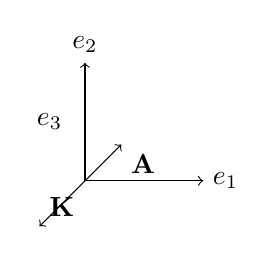
\begin{tikzpicture}[scale=1.5]
    \draw[->] (0,0,0) -- (1,0,0) node[right] {$e_1$};
    \draw[->] (0,0,0) -- (0,1,0) node[above] {$e_2$};
    \draw[->] (0,0,0) -- (0,0,1) node[above right] {$\mathbf{K}$};
    \draw[->] (0,0,0) -- (0.5,0.5,0.5) node[below right] {$\mathbf{A}$};

    \node at (-0.3,0.5,0) {$e_3$};
\end{tikzpicture}
  \caption[]{EJes}
  \labfig{fig:}
\end{marginfigure}

Otra base, también ortonormal, es 

$$
e_\pm = \frac{1}{\sqrt{2}} (\mathbf{E}(\mathbf{K}, 1) \pm i \mathbf{E}(\mathbf{K}, 2))
$$

Con $\mathbf{E}(\mathbf{K}, \lambda) \cdot \mathbf{E}(\mathbf{K}, \nu) = \delta_{\lambda\nu}$

Esta nueva base está relacionada con la helicidad y, por ejemplo, $e_+$ será un fotón de helicidad positiva.

Se puede construir un tensor energía-momento en esta teoría clásica

$$
\Theta^{\mu\nu} = \frac{\delta \mathcal{L}}{\delta(\partial_\mu A_\rho)} \partial^\nu A_\rho - g^{\mu\nu} \mathcal{L} \quad \Rightarrow \quad -F^{\mu\rho} \partial^\nu A_\rho + \frac{1}{4} g^{\mu\nu} F^2
$$

$$
\partial_\mu \Theta^{\mu\nu} = 0 \quad \Rightarrow \quad T^{\mu\nu} = \Theta^{\mu\nu} - \partial_\rho (F^{\rho\mu} A^\nu)
$$

$$A^{\mu\nu} = -F^{\mu\lambda} A_\lambda$$

Esto lo hacemos para construir un tensor simétrico.
\section{Cuantización covariante}

Imponer las condiciones gauge de radiación significaba perder la covariancia, por lo que ahora vamos a ver como se cuantizaria este campo sin imponer las condiciones del Gauge de radiación.

$$
\begin{cases}
\text{Gauge de radiación} & \phi = A^0 = 0 \\
\text{Gauge de Coulomb} & \nabla \cdot \mathbf{A} = 0 \\
\text{Gauge de Lorenz} & \partial_\mu A^\mu = 0
\end{cases}
$$

$$
\Box A^\mu = 0
$$


\subsection{Método de Gupta-Bleuler}

Ahora partimos de un lagrangiano diferente $\mathcal{L}' = \frac{1}{4} F^{\mu\nu} F_{\mu\nu} = \frac{1}{2} (\partial_\mu A^\nu)^2$.

$
\Pi^0 = \frac{\delta \mathcal{L}'}{\delta(\partial_0 A_0)} = -\partial_0 A^0 
$

$
\Pi^i = \frac{\delta \mathcal{L}'}{\delta(\partial_0 A_i)} = -F^{0i} = E^i
$

Ahora se cumple directamente que $\Box A^\mu = 0$.

Vamos a suponer una onda plana en la dirección $\hat{z}$ con $K^\mu = (\omega, 0, 0, \omega)$ en donde tendremos 4 polarizaciones $\epsilon^\mu(K, \lambda) = \epsilon^\mu_A(K) = \delta^\mu_\lambda$.

$
A^\mu = \sum_{\lambda = 0}^3 \int dK \left( \epsilon^\mu_{\mathbf{K}, \lambda} \hat{a}_{\mathbf{K}, \lambda} e^{-iKx} + \epsilon^{\ast \mu}_{\mathbf{K}, \lambda} \hat{a}_{\mathbf{K}, \lambda}^\dagger e^{iKx} \right)
$

Relaciones de conmutación

$
[\hat{A}^M(x, t), \hat{\Pi}^N(\mathbf{x}', t)] = i g^{\mu\nu} \delta(\mathbf{x} - \mathbf{x'})
$

Esto da lugar a estados de norma negativa

$
\langle \mathbf{K}', \lambda' = 0 | \mathbf{K}, \lambda = 0 \rangle < 0 
$

lo cual es inconsistente con la teoría, por lo que vamos a coger un subespacio del espacio de Fock $\mathcal{P} \subseteq \mathcal{F}$ tal que $|\psi\rangle, |\psi'\rangle \in \mathcal{P}$.

$ 
\langle \psi' | \partial_\mu \hat{A}^M |\psi\rangle = 0 
$

En este subespacio también se cumple que $ \partial_\mu \hat{A}^{M (+)} |\psi\rangle = 0 $.

$\hat{a}_{\mathbf{K},\lambda}$ y $\hat{a}^\dagger_{\mathbf{K},\lambda}$ son los operadores de creación y destrucción de fotones con momento $\mathbf{K}$ y polarización $\lambda$.

\subsubsection{Reglas de conmutación}

$$
[\hat{a}_{\mathbf{K},\lambda}, \hat{a}^\dagger_{\mathbf{K}',\lambda'}] = (2\pi)^3 \delta_{\lambda\lambda'} \delta(\mathbf{K} - \mathbf{K'})
$$

$$
[\hat{a}, \hat{a}] = [\hat{a}^\dagger, \hat{a}^\dagger] = 0
$$

$$
\hat{A}_i = \hat{\Pi}^i = E^i
$$

Ahora podemos obtener las reglas de conmutación del campo (como en los ejercicios):

$$
[\hat{A}^i(\mathbf{x}, t), \hat{E}^i(\mathbf{x}', t)] = -i \int \frac{dK}{(2\pi)^3} e^{i \mathbf{K} (\mathbf{x} - \mathbf{x'})} \left(K^i \left(\delta^{ij} - \frac{K^i K^j}{|\mathbf{K}|^2}\right)\right)
$$

Este término garantiza que $\nabla \cdot \mathbf{A} = 0$

$$
[\nabla \times \hat{A}, \mathbf{E}] = -i \int \frac{dK}{(2\pi)^3} e^{i \mathbf{K} (\mathbf{x} - \mathbf{x'})} K^i \left(\delta^{ij} - \frac{K^i K^j}{|\mathbf{K}|^2}\right) = 0
$$

\subsubsection{Estados de Fock}

$$
|0\rangle = \text{Estado de vacío} 
$$

$$
\hat{a}_{\mathbf{K},\lambda} |0\rangle = 0 \quad \hat{a}^\dagger_{\mathbf{K},\lambda} |0\rangle = |\mathbf{K}, \lambda \rangle 
$$

$$
H_0 \Rightarrow \hat{H}_0 = \frac{1}{2} \int dx (\mathbf{E}^2 + \mathbf{B}^2) = \sum_\lambda \int dK \, \omega_K \, \hat{a}^\dagger_{\mathbf{K},\lambda} \hat{a}_{\mathbf{K},\lambda}
$$

$$
\hat{\mathbf{P}} = \int dx \, \hat{\mathbf{E}} \times \hat{\mathbf{B}} = \sum_\lambda \int dK \, \mathbf{K} \, \hat{n}_{\mathbf{K},\lambda}
$$

Los estados que cumplen esta condición son las siguientes combinaciones:

\begin{itemize}
    \item \textbf{Estados transversales}
    $
    |\psi_T\rangle = \hat{a}^\dagger_T \hat{a}^\dagger_L |\phi\rangle \in \mathcal{P}
    $

    \item \textbf{Estados temporales}
    $
    |\phi\rangle = (\hat{a}^\dagger_\text{temp} - \hat{a}^\dagger_\text{long}) |0\rangle \in \mathcal{P}
    $

    $
    |\psi\rangle = |\psi_T\rangle + \lambda |\phi\rangle \quad \text{también son estados de este espacio}
    $
\end{itemize}

De esta forma, los estados físicos están contenidos.